% !TeX root = ../main.tex

\begingroup
\raggedbottom
\section{本章例题集}

\begin{workedexample}[由周期阶梯频谱反求序列]
  \label{ex:dtft-stepped-spectrum}
  已知 $X(\e^{\iu\omega})$ 以 $\pi$ 为周期。在 $|\omega|<\pi/2$ 内，
  \[
    X(\e^{\iu\omega})=
    \begin{cases}
      2,&|\omega|<\pi/8,\\
      1,&\pi/8<|\omega|<3\pi/8,\\
      0,&3\pi/8<|\omega|<\pi/2.
    \end{cases}
  \]
  跳跃点取左右值的平均数。求 $x[n]$，并说明哪些样值为零。题图见\cref{fig:ex-dtft-stepped-given}。
  \begin{figure}[H]
    \centering
    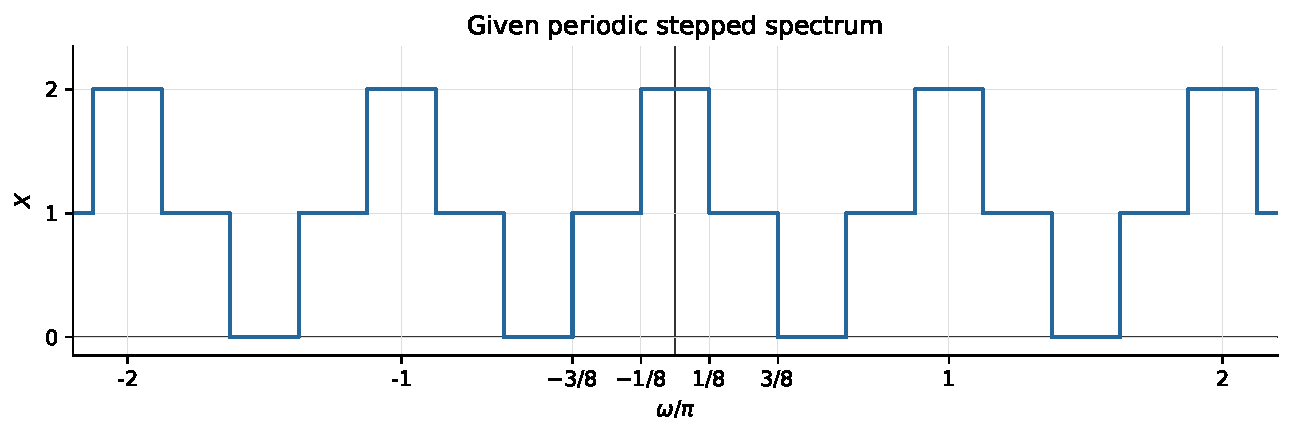
\includegraphics[width=0.84\textwidth]{07-dtft/examples/stepped-given.pdf}
    \caption{例题 \ref{ex:dtft-stepped-spectrum} 的已知频谱。图中在 $0$ 和整数倍 $\pi$ 附近各有一组阶梯。}
    \label{fig:ex-dtft-stepped-given}
  \end{figure}
\end{workedexample}

\begin{solution}
  先取一个以 $2\pi$ 为周期、只在零频附近有阶梯的频谱
  \[
    G(\omega)=R_{3\pi/8}(\omega)+R_{\pi/8}(\omega).
  \]
  由\cref{eq:dtft-sinc-pair}，其逆变换为
  \[
    g[n]=s_{3\pi/8}[n]+s_{\pi/8}[n],
    \qquad g[0]=\frac38+\frac18=\frac12.
  \]
  已知频谱由 $G(\omega)$ 与平移 $\pi$ 的 $G(\omega-\pi)$ 相加。此处可直接换元计算第二项：
  \[
    \frac1{2\pi}\int_{\alpha}^{\alpha+2\pi}
      G(\omega-\pi)\e^{\iu\omega n}\dd\omega
    =\e^{\iu\pi n}\frac1{2\pi}
      \int_{\alpha-\pi}^{\alpha+\pi}G(\nu)\e^{\iu\nu n}\dd\nu
    =(-1)^n g[n].
  \]
  积分长度保持 $2\pi$，可以使用任意基本区间。合并得到
  \[
    x[n]=[1+(-1)^n]\bigl(s_{3\pi/8}[n]+s_{\pi/8}[n]\bigr).
  \]
  写成不含 $0/0$ 的形式，
  \[
    \boxed{
    x[n]=
    \begin{cases}
      \displaystyle[1+(-1)^n]\,
        \frac{\sin(3\pi n/8)+\sin(\pi n/8)}{\pi n},&n\ne0,\\[5pt]
      1,&n=0.
    \end{cases}}
  \]
  全部奇数样值为零。对非零偶数 $n$，用
  \[
    \sin\frac{3\pi n}{8}+\sin\frac{\pi n}{8}
    =2\sin\frac{\pi n}{4}\cos\frac{\pi n}{8}
  \]
  可知 $n$ 为 $4$ 的非零整数倍时也为零；$n=4k+2$ 时两因子均非零。因此零样值恰好位于所有奇数及 $4$ 的非零整数倍处。
  中心值可由一个 $2\pi$ 周期的频谱面积核对：两组阶梯总面积为 $2\pi$，故 $x[0]=1$。样值见\cref{fig:ex-dtft-stepped-answer}。
  \begin{figure}[H]
    \centering
    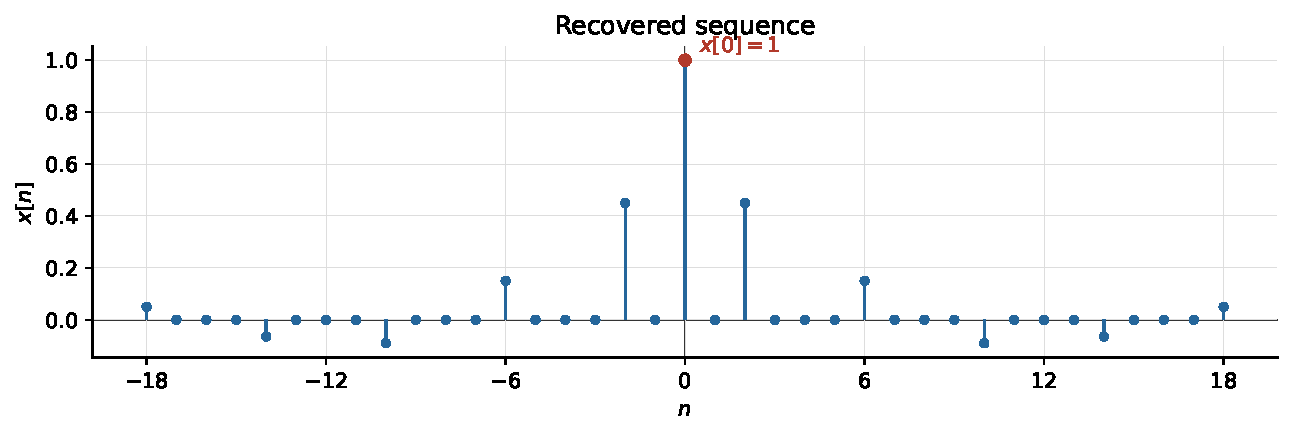
\includegraphics[width=0.84\textwidth]{07-dtft/examples/stepped-answer.pdf}
    \caption{例题 \ref{ex:dtft-stepped-spectrum} 的序列。除 $n=0$ 外，仅 $n=4k+2$ 处的样值非零；红点标出 $x[0]=1$。}
    \label{fig:ex-dtft-stepped-answer}
  \end{figure}
\end{solution}

\begin{technique}
  阶梯频谱可拆成不同半宽的矩形之和。反演时先选一个基本周期，确认该周期内包含几组副本；随后分别计算。若频谱每隔 $\pi$ 重复，积分中两份贡献在奇数 $n$ 处相消，可用来检查答案。零点样值另由频谱面积求出。
\end{technique}

\begin{workedexample}[高通矩形频谱的两种反演]
  \label{ex:dtft-highpass}
  已知频谱以 $2\pi$ 为周期，一个基本周期内为
  \[
    X(\e^{\iu\omega})=
    \begin{cases}
      0,&|\omega|<3\pi/4,\\
      1,&3\pi/4<|\omega|<\pi.
    \end{cases}
  \]
  跳跃点取平均值。求 $x[n]$，并分别用“补成全通带”和“平移低通矩形”两种方法计算。题图见\cref{fig:ex-dtft-highpass-given}。
  \begin{figure}[H]
    \centering
    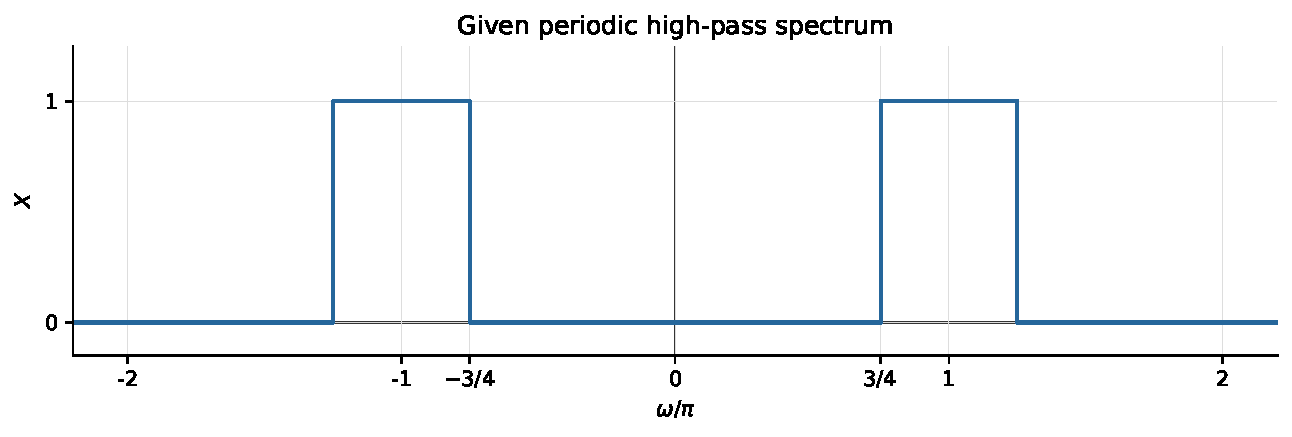
\includegraphics[width=0.84\textwidth]{07-dtft/examples/highpass-given.pdf}
    \caption{例题 \ref{ex:dtft-highpass} 的周期频谱。每个主周期的通带位于 $\pm\pi$ 附近。}
    \label{fig:ex-dtft-highpass-given}
  \end{figure}
\end{workedexample}

\begin{solution}
  在一个主周期内补成恒为 $1$ 的频谱，
  \[
    X(\e^{\iu\omega})=1-R_{3\pi/4}(\omega).
  \]
  利用 $\impulse[n]\fourierpair1$ 得到
  \[
    x[n]=\impulse[n]-s_{3\pi/4}[n]
    =\begin{cases}
      -\dfrac{\sin(3\pi n/4)}{\pi n},&n\ne0,\\[4pt]
      \dfrac14,&n=0.
    \end{cases}
  \]
  这里频域恒为 $1$ 的背景对应 $\impulse[n]$。

  另一种表示为 $X(\e^{\iu\omega})=R_{\pi/4}(\omega-\pi)$。矩形越过基本区间右边界的部分，按周期延拓出现在左边界附近。对逆变换作与上一题相同的换元，可得
  \[
    x[n]=(-1)^n s_{\pi/4}[n].
  \]
  两个答案在 $n=0$ 处都为 $1/4$。对非零整数 $n$，
  \[
    \sin\frac{3\pi n}{4}
    =\sin\left(\pi n-\frac{\pi n}{4}\right)
    =-(-1)^n\sin\frac{\pi n}{4},
  \]
  故也完全相同。一个主周期的通带总宽为 $\pi/2$，再次给出
  $x[0]=(\pi/2)/(2\pi)=1/4$。答案见\cref{fig:ex-dtft-highpass-answer}。
  \begin{figure}[H]
    \centering
    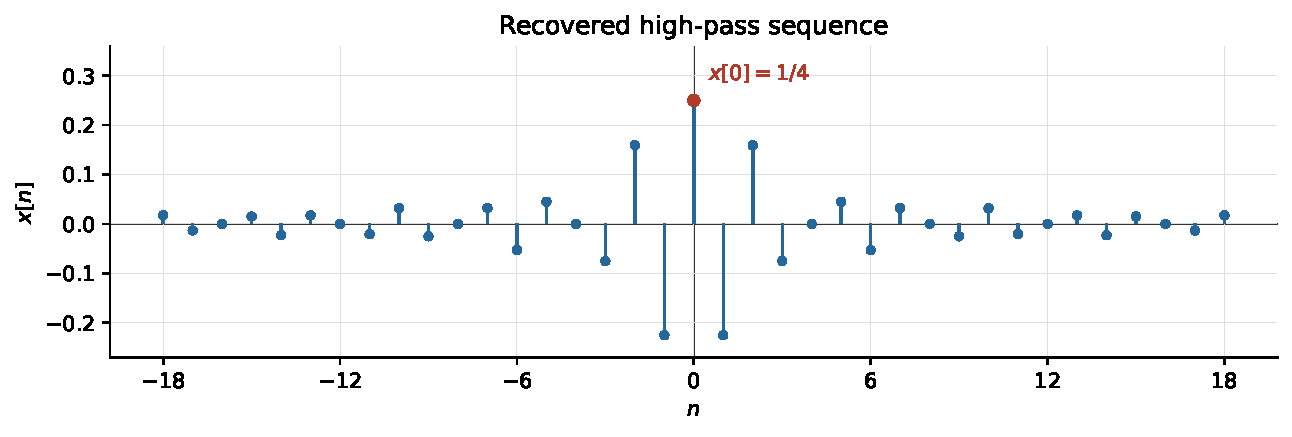
\includegraphics[width=0.84\textwidth]{07-dtft/examples/highpass-answer.pdf}
    \caption{例题 \ref{ex:dtft-highpass} 的序列，两种表示逐点相同。}
    \label{fig:ex-dtft-highpass-answer}
  \end{figure}
\end{solution}

\begin{technique}
  高频通带跨过 $\pm\pi$ 边界时，可减去零频附近的低通矩形，也可把低通矩形平移半个周期。比较两个时域表达式时，分别检查 $n=0$ 与非零整数 $n$；只用正弦恒等式约分，容易漏掉零点的单位冲激项。
\end{technique}
\begin{workedexample}[只有主值分式时的反演]
  \label{ex:dtft-principal-sum}
  已知
  \[
    Z(\e^{\iu\omega})
    =\left(\operatorname{pv}\frac1{1-\e^{-\iu\omega}}\right)
      \frac{\sin(5\omega/2)}{\sin(\omega/2)}.
  \]
  第二因子在 $\omega=2m\pi$ 处补值为 $5$；第一因子只含主值项。求 $z[n]$，并与五点矩形的真正累加比较。两因子的频谱见\cref{fig:ex-dtft-principal-given}。
  \begin{figure}[H]
    \centering
    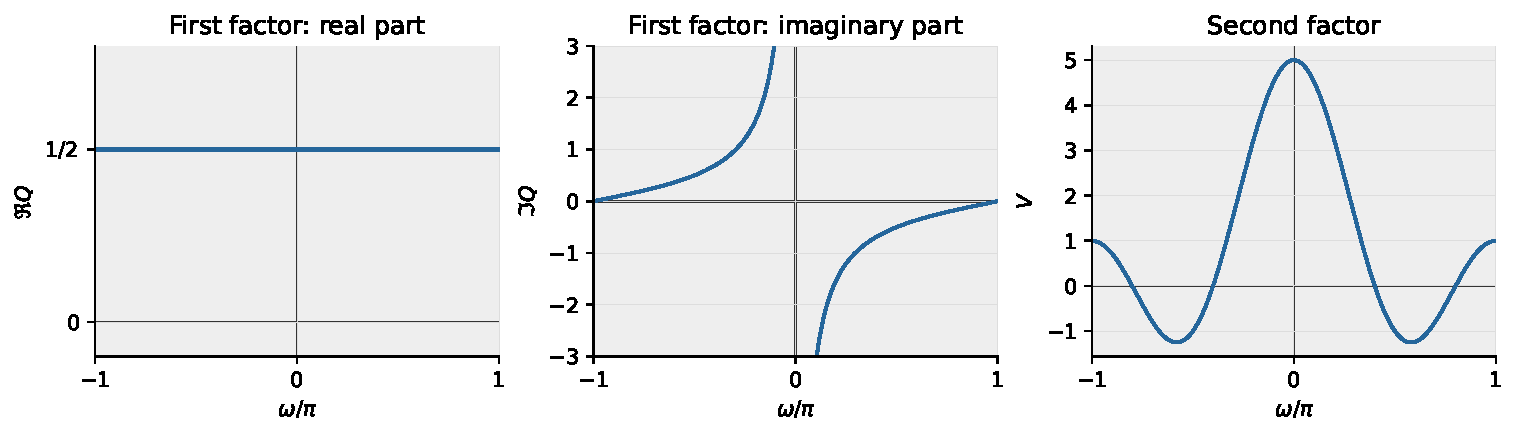
\includegraphics[width=0.92\textwidth]{07-dtft/examples/principal-given.pdf}
    \caption{例题 \ref{ex:dtft-principal-sum} 的两个频域因子。左列分式的实部为 $1/2$、虚部为周期主值余切；右列为五点矩形的带符号频谱。}
    \label{fig:ex-dtft-principal-given}
  \end{figure}
\end{workedexample}

\begin{solution}
  由\cref{eq:dtft-step-without-dc,eq:dtft-rectangle}，两个因子的反演分别为
  \[
    q[n]=\stepfun[n]-\frac12
      =\begin{cases}-1/2,&n<0,\\1/2,&n\ge0,\end{cases}
    \qquad
    v[n]=\begin{cases}1,&-2\le n\le2,\\0,&\text{其他}.\end{cases}
  \]
  因为频域相乘对应时域卷积，
  \[
    z[n]=\sum_{k=-2}^{2}v[k]q[n-k].
  \]
  固定 $v[k]$，先把 $q[k]$ 翻转为 $q[-k]$，此时 $k\le0$ 处为 $1/2$、$k>0$ 处为 $-1/2$；再平移为 $q[n-k]$，其分界点位于 $k=n$。每次 $n$ 增加 $1$，分界点向右移一格，使新增一个矩形样值与 $+1/2$ 配对。相乘时按同一横坐标 $k$ 对齐，配对见\cref{fig:ex-dtft-principal-alignment}。
  \begin{figure}[H]
    \centering
    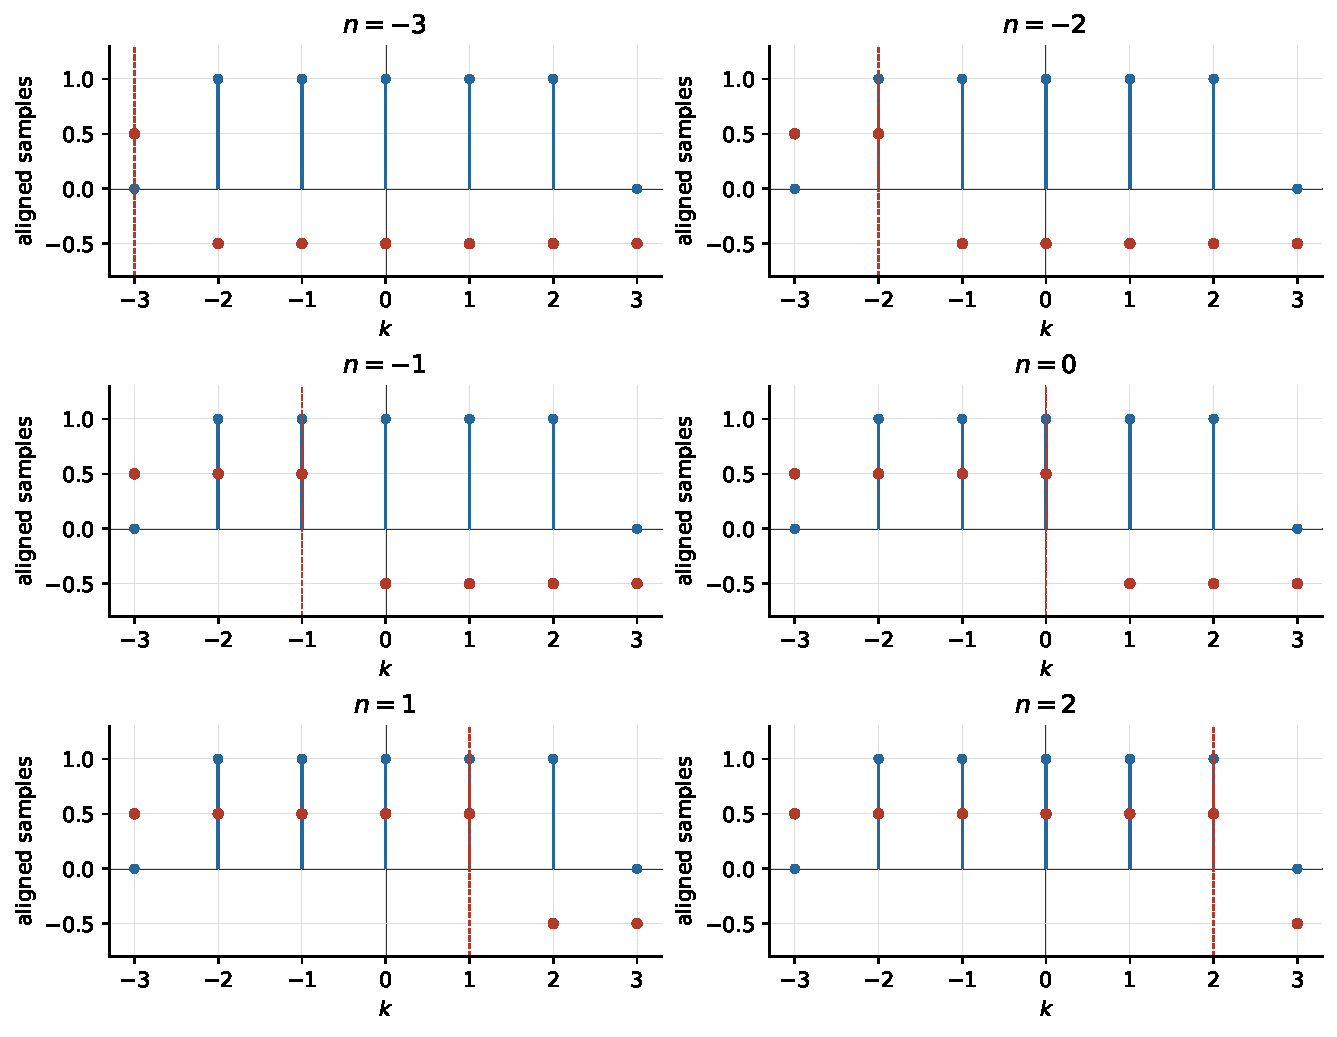
\includegraphics[width=0.92\textwidth]{07-dtft/examples/principal-alignment.pdf}
    \caption{例题 \ref{ex:dtft-principal-sum} 的翻转平移配对。蓝色竖线为 $v[k]$，红点为 $q[n-k]$，两者按 $k=-2,\ldots,2$ 对齐；虚线标出平移后的分界点 $k=n$。}
    \label{fig:ex-dtft-principal-alignment}
  \end{figure}

  先逐点求积。五个矩形样值均为 $1$，下表的五项依次对应 $k=-2,-1,0,1,2$：
  \begin{center}
    \renewcommand{\arraystretch}{1.4}
    \begin{tabular}{ccl}
      \hline
      $n$ & $z[n]$ & 五个乘积之和\\
      \hline
      $-3$ & $-5/2$ & $1(-\tfrac12)+1(-\tfrac12)+1(-\tfrac12)+1(-\tfrac12)+1(-\tfrac12)$\\
      $-2$ & $-3/2$ & $1(\tfrac12)+1(-\tfrac12)+1(-\tfrac12)+1(-\tfrac12)+1(-\tfrac12)$\\
      $-1$ & $-1/2$ & $1(\tfrac12)+1(\tfrac12)+1(-\tfrac12)+1(-\tfrac12)+1(-\tfrac12)$\\
      $0$ & $1/2$ & $1(\tfrac12)+1(\tfrac12)+1(\tfrac12)+1(-\tfrac12)+1(-\tfrac12)$\\
      $1$ & $3/2$ & $1(\tfrac12)+1(\tfrac12)+1(\tfrac12)+1(\tfrac12)+1(-\tfrac12)$\\
      $2$ & $5/2$ & $1(\tfrac12)+1(\tfrac12)+1(\tfrac12)+1(\tfrac12)+1(\tfrac12)$\\
      $3$ & $5/2$ & $1(\tfrac12)+1(\tfrac12)+1(\tfrac12)+1(\tfrac12)+1(\tfrac12)$\\
      \hline
    \end{tabular}
  \end{center}
  对 $n\le-3$，五项全为负；对 $n\ge2$，五项全为正。对 $-2\le n\le2$，条件 $k\le n$ 给出 $n+3$ 个正项，另有 $2-n$ 个负项，于是
  \[
    z[n]=\frac{n+3}{2}-\frac{2-n}{2}=n+\frac12.
  \]
  合写为
  \[
    \boxed{
    z[n]=
    \begin{cases}
      -5/2,&n\le-3,\\
      n+1/2,&-2\le n\le2,\\
      5/2,&n\ge3.
    \end{cases}}
  \]
  其中 $n=2$ 已经进入右端平台。

  真正累加 $c[n]=\sum_{k=-\infty}^{n}v[k]$，则
  \[
    c[n]=
    \begin{cases}
      0,&n\le-3,\\
      n+3,&-2\le n\le2,\\
      5,&n\ge3.
    \end{cases}
    \qquad z[n]=c[n]-\frac52.
  \]
  因为 $V(\e^{\iu0})=5$，$c[n]$ 的频谱比题给频谱多
  $5\pi\sum_m\impulse(\omega-2m\pi)$，对应时域常数 $5/2$。两种结果见\cref{fig:ex-dtft-principal-answer}。
  \begin{figure}[H]
    \centering
    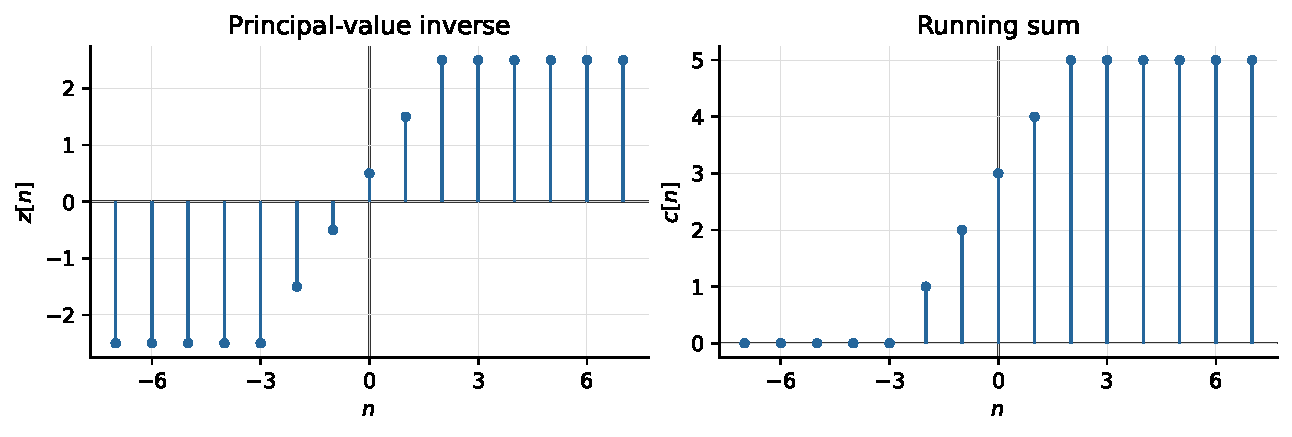
\includegraphics[width=0.86\textwidth]{07-dtft/examples/principal-answer.pdf}
    \caption{例题 \ref{ex:dtft-principal-sum} 的结果。主值分式反演与真正累加相差常数 $5/2$，两者的一阶差分相同。}
    \label{fig:ex-dtft-principal-answer}
  \end{figure}
\end{solution}

\begin{technique}
  先辨认阶跃频谱是否包含周期冲激。只有主值分式时，反演为 $u[n]-1/2$。与有限矩形卷积，可先按平移分界点逐个列乘积，再数正、负项归纳分段式；用左端平台、右端平台和 $n=0$ 三处核对，能检查是否误加了累加常数。
\end{technique}

\begin{workedexample}[指数输入通过指数脉冲响应的系统]
  \label{ex:dtft-exponential-convolution}
  离散 LTI 系统的单位脉冲响应为 $h[n]=\alpha^n\stepfun[n]$，输入为 $x[n]=\beta^n\stepfun[n]$，其中 $|\alpha|<1$、$|\beta|<1$。求输出，分别讨论 $\alpha=\beta$ 与 $\alpha\ne\beta$。一组已知样值见\cref{fig:ex-dtft-exponential-given}。
  \begin{figure}[H]
    \centering
    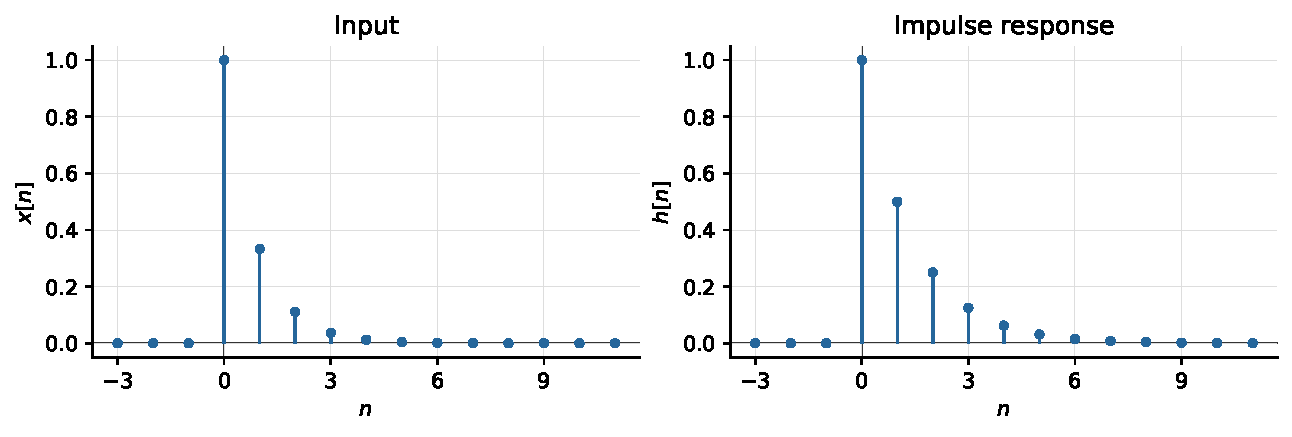
\includegraphics[width=0.86\textwidth]{07-dtft/examples/exponential-given.pdf}
    \caption{例题 \ref{ex:dtft-exponential-convolution} 的输入与脉冲响应示意，取 $\beta=1/3$、$\alpha=1/2$。}
    \label{fig:ex-dtft-exponential-given}
  \end{figure}
\end{workedexample}

\begin{solution}
  先变换再相乘：
  \[
    X(\e^{\iu\omega})=\frac1{1-\beta\e^{-\iu\omega}},\qquad
    H(\e^{\iu\omega})=\frac1{1-\alpha\e^{-\iu\omega}},
  \]
  \[
    Y(\e^{\iu\omega})
      =\frac1{(1-\alpha\e^{-\iu\omega})(1-\beta\e^{-\iu\omega})}.
  \]
  若 $\alpha=\beta$，分母为二次重复因子。用\cref{eq:dtft-repeated-pole} 的 $r=2$ 情形，
  \[
    \boxed{y[n]=(n+1)\alpha^n\stepfun[n]}.
  \]
  若 $\alpha\ne\beta$，设
  \[
    Y=\frac{A}{1-\alpha\e^{-\iu\omega}}
       +\frac{B}{1-\beta\e^{-\iu\omega}}.
  \]
  通分后比较常数与 $\e^{-\iu\omega}$ 的系数：
  \[
    A+B=1,\qquad A\beta+B\alpha=0,
    \qquad
    A=\frac{\alpha}{\alpha-\beta},\quad
    B=-\frac{\beta}{\alpha-\beta}.
  \]
  逐项反演，
  \[
    \boxed{
    y[n]=\left(\frac{\alpha}{\alpha-\beta}\alpha^n
        -\frac{\beta}{\alpha-\beta}\beta^n\right)\stepfun[n]
      =\frac{\alpha^{n+1}-\beta^{n+1}}{\alpha-\beta}\stepfun[n]}.
  \]
  各式在 $n<0$ 时直接规定为零，避免零参数的负次幂。

  用时域前几个样值核对。两个序列在负下标都为零；翻转 $h[k]$ 为 $h[-k]$ 后，再平移为 $h[n-k]$，与 $x[k]$ 同下标配对：
  \begin{align*}
    y[0]&=x[0]h[0]=1,\\
    y[1]&=x[0]h[1]+x[1]h[0]=\alpha+\beta,\\
    y[2]&=x[0]h[2]+x[1]h[1]+x[2]h[0]
      =\alpha^2+\alpha\beta+\beta^2.
  \end{align*}
  每次向右平移一格，新增一个乘积；由 $k\ge0$ 与 $n-k\ge0$ 得到一般范围 $0\le k\le n$。$n\ge0$ 时，
  \[
    y[n]=\sum_{k=0}^{n}\beta^k\alpha^{n-k}.
  \]
  $\alpha=\beta$ 时每项均为 $\alpha^n$，共 $n+1$ 项；不等时的有限等比和给出同一答案。两种情况的输出示意见\cref{fig:ex-dtft-exponential-answer}。
  \begin{figure}[H]
    \centering
    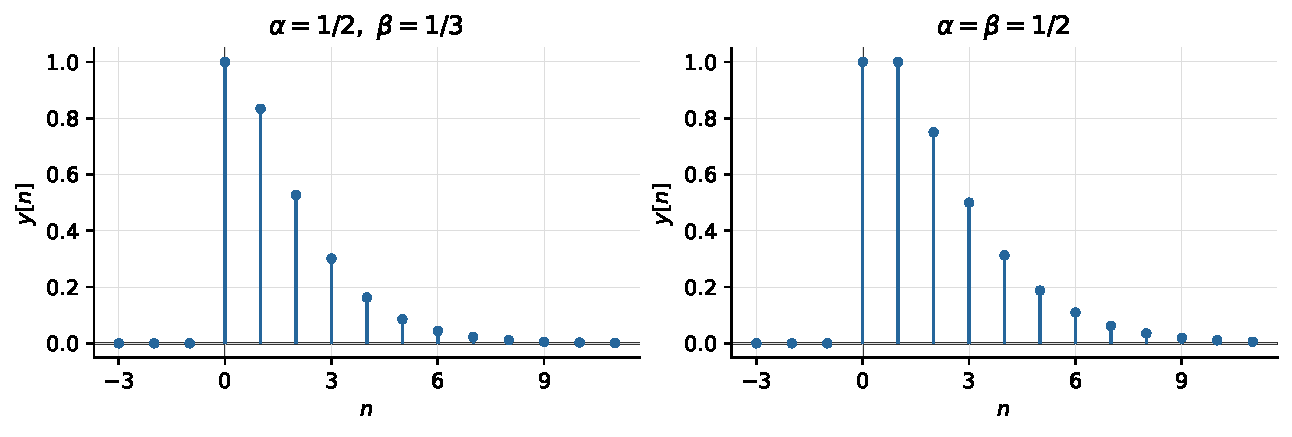
\includegraphics[width=0.86\textwidth]{07-dtft/examples/exponential-answer.pdf}
    \caption{例题 \ref{ex:dtft-exponential-convolution} 的两种输出：左图 $\alpha=1/2,\beta=1/3$，右图 $\alpha=\beta=1/2$。}
    \label{fig:ex-dtft-exponential-answer}
  \end{figure}
\end{solution}

\begin{technique}
  先判断两个指数参数是否相等。不等时按一次因子拆部分分式；相等时使用多项式加权指数变换对。求得一般式后，再代入 $n=0,1,2$ 与直接卷积核对；含 $\alpha-\beta$ 的分母不能用于参数相等的情况。
\end{technique}

\begin{workedexample}[由一组输入输出反求系统]
  \label{ex:dtft-identify-system}
  已知离散 LTI 系统的一组输入输出为
  \[
    x[n]=\left(\frac12\right)^n\stepfun[n],\qquad
    y[n]=3\left(\frac12\right)^n\stepfun[n]
        -2\left(\frac13\right)^n\stepfun[n].
  \]
  求 $H(\e^{\iu\omega})$ 与 $h[n]$。样值见\cref{fig:ex-dtft-identify-given}。
  \begin{figure}[H]
    \centering
    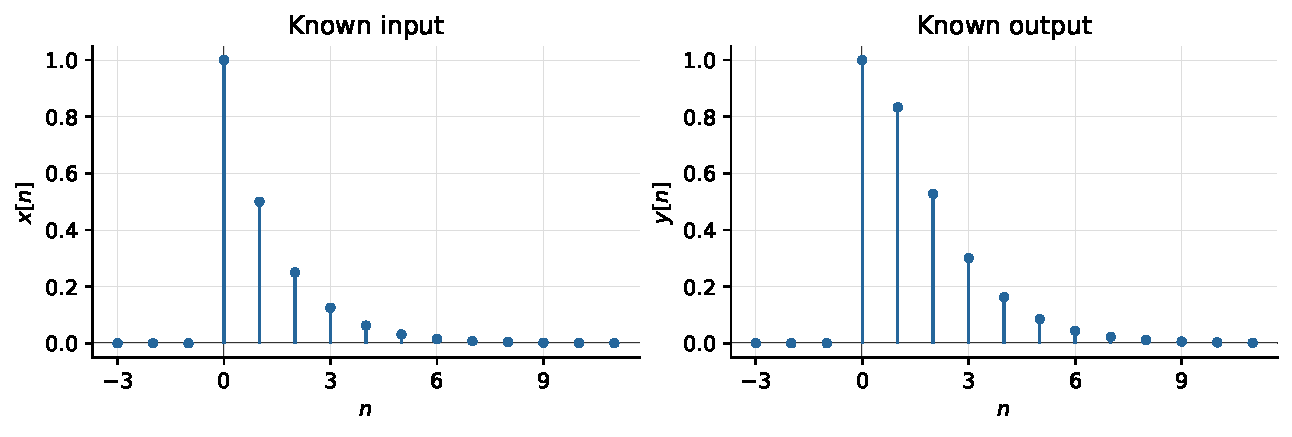
\includegraphics[width=0.86\textwidth]{07-dtft/examples/identify-given.pdf}
    \caption{例题 \ref{ex:dtft-identify-system} 的已知输入与输出。两者在负下标均为零。}
    \label{fig:ex-dtft-identify-given}
  \end{figure}
\end{workedexample}

\begin{solution}
  先分别变换：
  \[
    X=\frac1{1-\tfrac12\e^{-\iu\omega}},\qquad
    Y=\frac3{1-\tfrac12\e^{-\iu\omega}}
       -\frac2{1-\tfrac13\e^{-\iu\omega}}.
  \]
  通分得到
  \[
    Y=\frac{3(1-\tfrac13\e^{-\iu\omega})
               -2(1-\tfrac12\e^{-\iu\omega})}
              {(1-\tfrac12\e^{-\iu\omega})(1-\tfrac13\e^{-\iu\omega})}
      =\frac1{(1-\tfrac12\e^{-\iu\omega})(1-\tfrac13\e^{-\iu\omega})}.
  \]
  因为 $X$ 对所有实数 $\omega$ 均非零，可在整个频率轴上相除：
  \[
    H=\frac{Y}{X}
      =\frac1{1-\tfrac13\e^{-\iu\omega}},
    \qquad
    \boxed{h[n]=\left(\frac13\right)^n\stepfun[n]}.
  \]
  所得系统因果且稳定。零点样值满足 $y[0]=x[0]h[0]=1$；下一点为
  $y[1]=x[0]h[1]+x[1]h[0]=1/3+1/2=5/6$，与题给表达式一致。脉冲响应与幅度响应见\cref{fig:ex-dtft-identify-answer}。
  \begin{figure}[H]
    \centering
    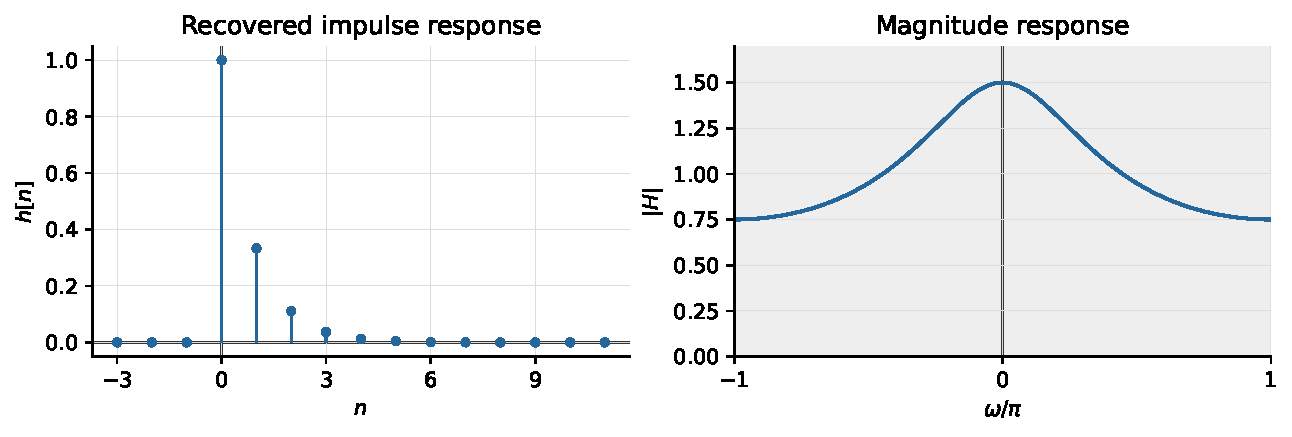
\includegraphics[width=0.86\textwidth]{07-dtft/examples/identify-answer.pdf}
    \caption{例题 \ref{ex:dtft-identify-system} 的脉冲响应与幅度响应，零频增益为 $3/2$。}
    \label{fig:ex-dtft-identify-answer}
  \end{figure}
\end{solution}

\begin{technique}
  反求系统时先化简 $Y$，再除以 $X$，并检查 $X$ 的零点。约分完成后才按已知变换对反演；最后用最前面的卷积样值核对，能发现部分分式的系数错误。
\end{technique}

\begin{workedexample}[差分方程与重复因子的反演]
  \label{ex:dtft-difference-equation}
  因果、初始静止的离散 LTI 系统满足
  \[
    y[n]-\frac16y[n-1]-\frac16y[n-2]=x[n].
  \]
  求频率响应和单位脉冲响应；再求 $x[n]=(1/2)^n\stepfun[n]$ 时的零状态响应。输入见\cref{fig:ex-dtft-equation-given}。
  \begin{figure}[H]
    \centering
    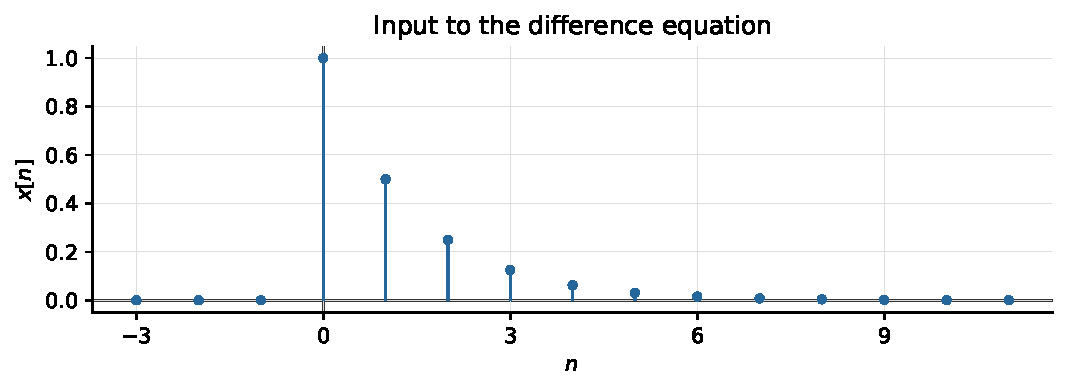
\includegraphics[width=0.76\textwidth]{07-dtft/examples/equation-given.pdf}
    \caption{例题 \ref{ex:dtft-difference-equation} 的指数输入，$x[0]=1$，负下标样值为零。}
    \label{fig:ex-dtft-equation-given}
  \end{figure}
\end{workedexample}

\begin{solution}
  将每一项分别变换：
  \[
    Y-\frac16\e^{-\iu\omega}Y
       -\frac16\e^{-2\iu\omega}Y=X.
  \]
  提出 $Y$ 并因式分解，
  \[
    H=\frac1{1-\tfrac16\e^{-\iu\omega}-\tfrac16\e^{-2\iu\omega}}
      =\frac1{(1-\tfrac12\e^{-\iu\omega})(1+\tfrac13\e^{-\iu\omega})}.
  \]
  设 $H=A/(1-\tfrac12\e^{-\iu\omega})+B/(1+\tfrac13\e^{-\iu\omega})$。通分后
  \[
    A+B=1,\qquad \frac A3-\frac B2=0
    \quad\Longrightarrow\quad A=\frac35,\quad B=\frac25.
  \]
  因果条件选取右侧序列，两个参数的模都小于 $1$：
  \[
    \boxed{h[n]=\frac35\left(\frac12\right)^n\stepfun[n]
                    +\frac25\left(-\frac13\right)^n\stepfun[n]}.
  \]
  它绝对可和，普通 DTFT 存在。代入脉冲输入递推核对：
  \[
    h[0]=1,\qquad h[1]=\frac16,\qquad
    h[2]=\frac16h[1]+\frac16h[0]=\frac7{36}.
  \]

  给定指数输入后，
  \[
    Y=HX
      =\frac1{(1-\tfrac12\e^{-\iu\omega})^2(1+\tfrac13\e^{-\iu\omega})}.
  \]
  输入使第一个因子重复，部分分式须包含两种次数：
  \[
    Y=\frac{C}{(1-\tfrac12\e^{-\iu\omega})^2}
      +\frac{D}{1-\tfrac12\e^{-\iu\omega}}
      +\frac{E}{1+\tfrac13\e^{-\iu\omega}}.
  \]
  为解系数，暂记 $q=\e^{-\iu\omega}$。清除分母后得到多项式恒等式
  \[
    1=C(1+q/3)+D(1-q/2)(1+q/3)+E(1-q/2)^2.
  \]
  在这一恒等式中代入 $q=2$、$q=-3$、$q=0$：
  \[
    C=\frac35,\qquad E=\frac4{25},\qquad
    D=1-C-E=\frac6{25}.
  \]
  这里代入的是多项式变量，$q=2,-3$ 用于求系数，不代表实频率点。

  按\cref{eq:dtft-repeated-pole} 反演重复因子，再合并其余两项：
  \[
    \boxed{
    y[n]=\left[
      \frac35(n+1)\left(\frac12\right)^n
      +\frac6{25}\left(\frac12\right)^n
      +\frac4{25}\left(-\frac13\right)^n
    \right]\stepfun[n]}.
  \]
  负下标直接取零。用原差分方程核对初始几项：
  \begin{align*}
    y[0]&=x[0]=1,\\
    y[1]&=x[1]+\frac16y[0]=\frac12+\frac16=\frac23,\\
    y[2]&=x[2]+\frac16y[1]+\frac16y[0]
      =\frac14+\frac19+\frac16=\frac{19}{36}.
  \end{align*}
  结果与反演式一致，脉冲响应及输出见\cref{fig:ex-dtft-equation-answer}。
  \begin{figure}[H]
    \centering
    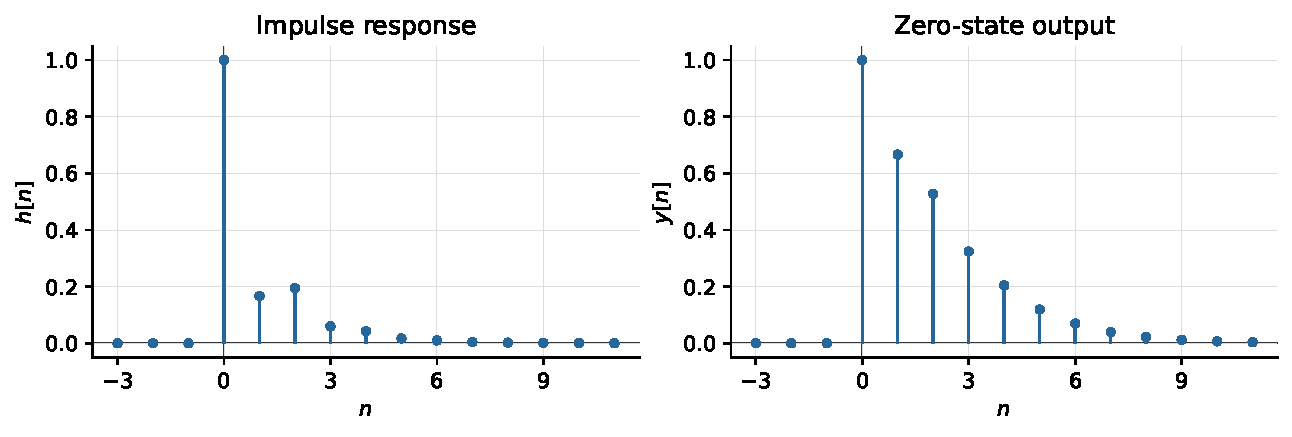
\includegraphics[width=0.86\textwidth]{07-dtft/examples/equation-answer.pdf}
    \caption{例题 \ref{ex:dtft-difference-equation} 的脉冲响应与指数输入的零状态输出。}
    \label{fig:ex-dtft-equation-answer}
  \end{figure}
\end{solution}

\begin{technique}
  先由差分方程得到 $H$，再求 $h$；输入确定后重新检查 $Y=HX$ 的因子次数。二次重复因子必须同时保留二次项和一次项。系数可在清除分母后的多项式恒等式中求出，反演后用原递推式检查 $n=0,1,2$，并确认负下标符合初始静止条件。
\end{technique}
\begin{workedexample}[窄 sinc 平方的三角频谱]
  \label{ex:dtft-sinc-square-narrow}
  求 $z[n]=s_{\pi/4}^2[n]$ 的 DTFT，其中 $s_{\pi/4}[0]=1/4$，所以 $z[0]=1/16$。序列见\cref{fig:ex-dtft-square-narrow-given}。
  \begin{figure}[H]
    \centering
    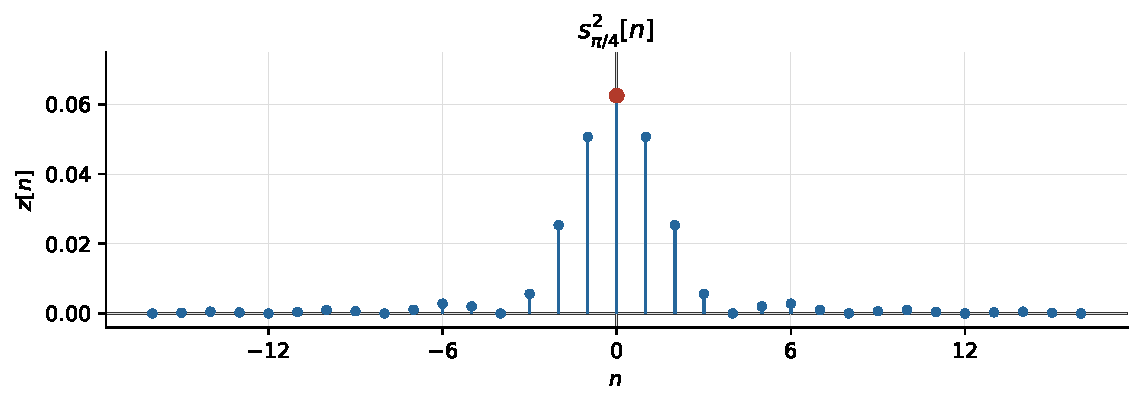
\includegraphics[width=0.82\textwidth]{07-dtft/examples/square-narrow-given.pdf}
    \caption{例题 \ref{ex:dtft-sinc-square-narrow} 的序列。sinc 的零点取极限值后再平方。}
    \label{fig:ex-dtft-square-narrow-given}
  \end{figure}
\end{workedexample}

\begin{solution}
  $s_{\pi/4}$ 对应高度 $1$、半宽 $\pi/4$ 的周期矩形。先截取中央两份矩形做普通卷积；它们的重叠长度为
  \[
    C_0(\omega)=
    \begin{cases}
      \pi/2-|\omega|,&|\omega|\le\pi/2,\\
      0,&|\omega|>\pi/2.
    \end{cases}
  \]
  支撑尚未越过 $\pm\pi$，周期副本在主周期内不重叠。乘以 $1/(2\pi)$ 后，
  \[
    \boxed{Z(\e^{\iu\omega})=
      \begin{cases}
        \displaystyle\frac14-\frac{|\omega|}{2\pi},
            &|\omega|\le\pi/2,\\
        0,&\pi/2<|\omega|\le\pi,
      \end{cases}}
  \]
  再以 $2\pi$ 为周期延拓，见\cref{fig:ex-dtft-square-narrow-answer}。中央高度为 $1/4$；一个三角形的面积为 $\pi/8$，除以 $2\pi$ 后得 $1/16$，与 $z[0]$ 一致。零频值 $Z(1)=1/4$ 则是全部样值的和，与 $z[0]$ 不同。
  \begin{figure}[H]
    \centering
    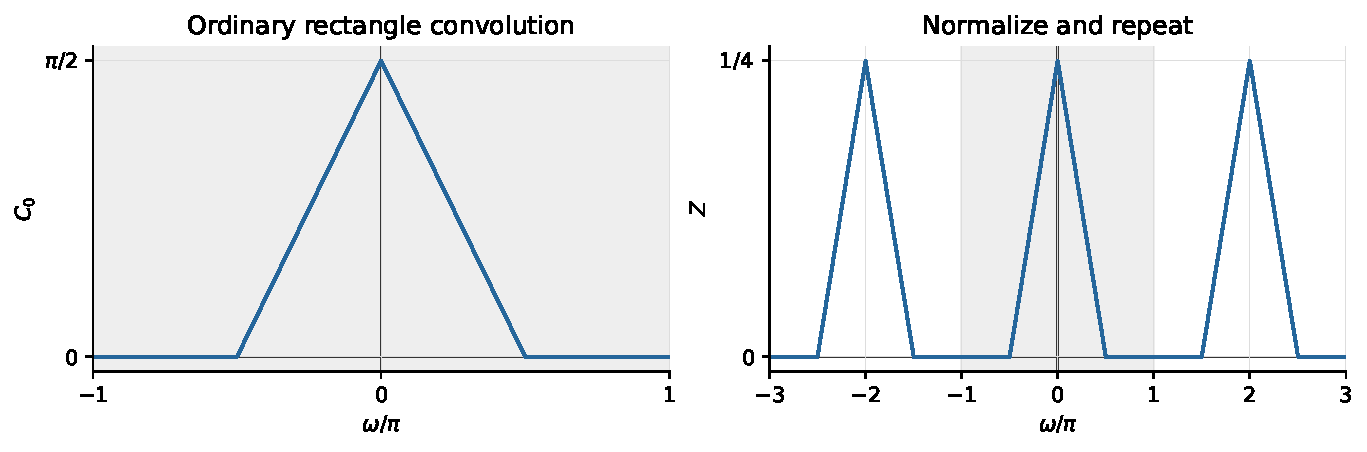
\includegraphics[width=0.90\textwidth]{07-dtft/examples/square-narrow-answer.pdf}
    \caption{例题 \ref{ex:dtft-sinc-square-narrow}：两个单位矩形普通卷积得到峰值 $\pi/2$ 的三角形，再乘 $1/(2\pi)$ 并周期延拓。}
    \label{fig:ex-dtft-square-narrow-answer}
  \end{figure}
\end{solution}

\begin{technique}
  矩形卷积先读重叠长度，确定三角形的底宽与峰值，再乘归一化系数。用频谱面积检查零点样值，用频谱零频值检查全序列求和；这两种核对不能混用。
\end{technique}

\begin{workedexample}[低通与高通三角频谱的反演]
  \label{ex:dtft-triangle-inverse}
  两个频谱均以 $2\pi$ 为周期。主周期内，
  \[
    G(\omega)=
    \begin{cases}
      1-4|\omega|/\pi,&|\omega|\le\pi/4,\\
      0,&\pi/4<|\omega|\le\pi,
    \end{cases}
  \]
  \[
    Q(\omega)=
    \begin{cases}
      0,&|\omega|<3\pi/4,\\
      4|\omega|/\pi-3,&3\pi/4\le|\omega|\le\pi.
    \end{cases}
  \]
  求对应序列 $g[n]$、$q[n]$。题图见\cref{fig:ex-dtft-triangle-given}。
  \begin{figure}[H]
    \centering
    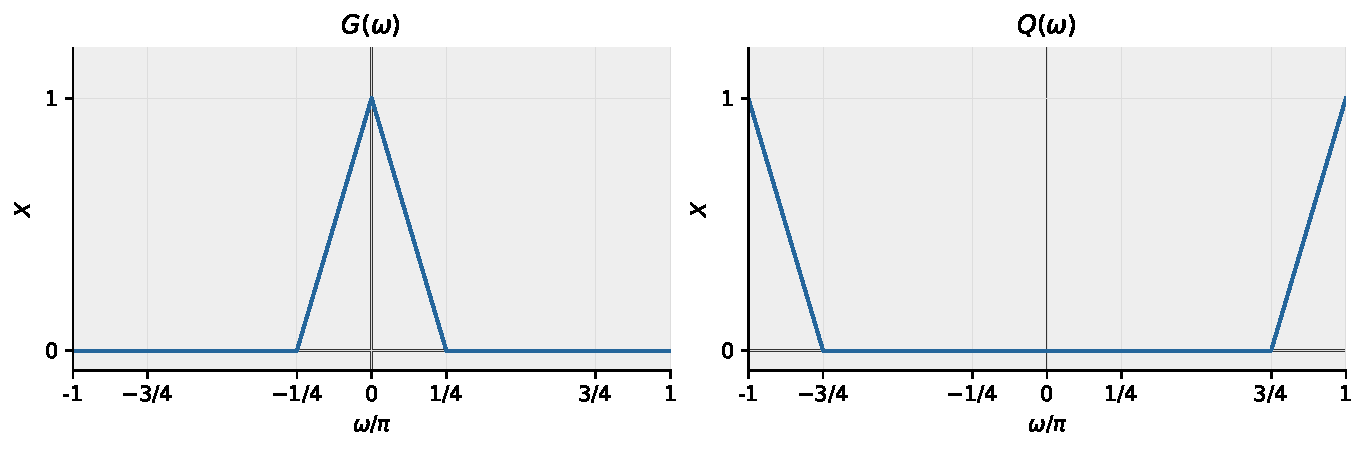
\includegraphics[width=0.90\textwidth]{07-dtft/examples/triangle-given.pdf}
    \caption{例题 \ref{ex:dtft-triangle-inverse} 的两种频谱。高通三角形的两半在主周期边界连接，$\pi$ 与 $-\pi$ 表示同一频率。}
    \label{fig:ex-dtft-triangle-given}
  \end{figure}
\end{workedexample}

\begin{solution}
  先求 $G$。两个半宽 $\pi/8$ 的单位矩形做普通卷积得到底边端点为 $\pm\pi/4$、峰值为 $\pi/4$ 的三角形。经 $1/(2\pi)$ 归一化后，峰值为 $1/8$；再乘 $8$ 就得到 $G$。于是
  \[
    \boxed{g[n]=8s_{\pi/8}^2[n]},\qquad
    g[0]=8\left(\frac18\right)^2=\frac18.
  \]
  $G$ 的面积为 $\pi/4$，逆变换的零点样值也是 $1/8$。

  高通频谱满足 $Q(\omega)=G(\omega-\pi)$。由频移性质，
  \[
    \boxed{q[n]=(-1)^ng[n]=8(-1)^ns_{\pi/8}^2[n]},\qquad q[0]=\frac18.
  \]
  两个序列的绝对值相同；高通序列的奇数样值反号，偶数样值不变，见\cref{fig:ex-dtft-triangle-answer}。低通谱的 $G(0)=1$，故 $\sum_n g[n]=1$；高通谱的 $Q(0)=0$，故 $\sum_n q[n]=0$，与交替符号相符。
  \begin{figure}[H]
    \centering
    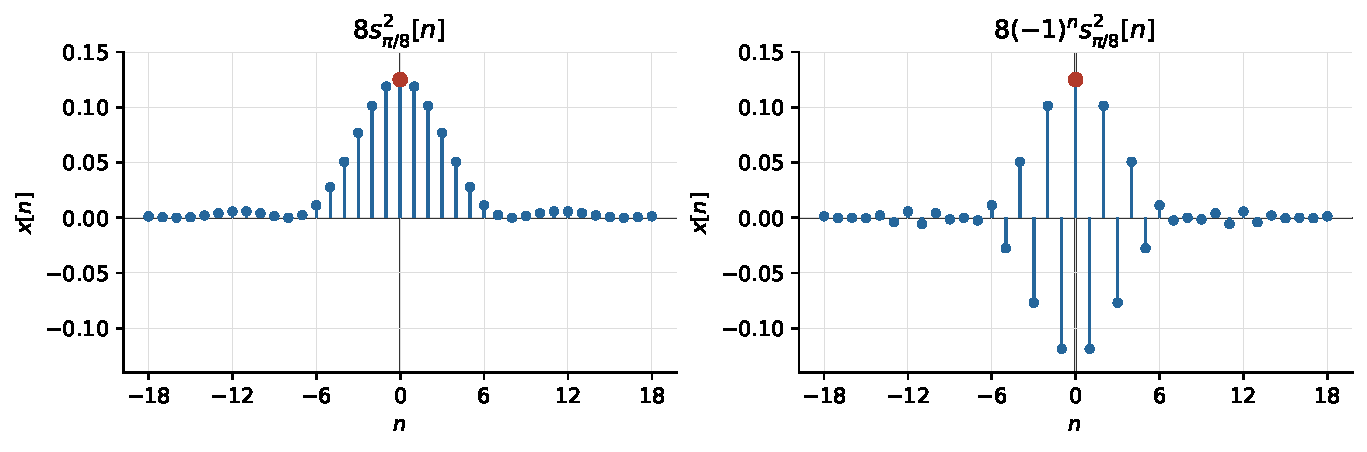
\includegraphics[width=0.90\textwidth]{07-dtft/examples/triangle-answer.pdf}
    \caption{例题 \ref{ex:dtft-triangle-inverse} 的答案。乘 $(-1)^n$ 改变样值符号，对应三角频谱平移 $\pi$。}
    \label{fig:ex-dtft-triangle-answer}
  \end{figure}
\end{solution}

\begin{technique}
  反演三角频谱时，先将半宽减半以构造两个矩形，再检查峰值所需的比例系数。高通图若是低通图在周期边界处的平移，可直接用 $(-1)^n$，并单独核对 $n=0$。
\end{technique}

\begin{workedexample}[宽 sinc 平方与周期重叠]
  \label{ex:dtft-sinc-square-wide}
  求 $z[n]=s_{3\pi/4}^2[n]$ 的 DTFT，零点定义为 $z[0]=9/16$。题图见\cref{fig:ex-dtft-square-wide-given}。
  \begin{figure}[H]
    \centering
    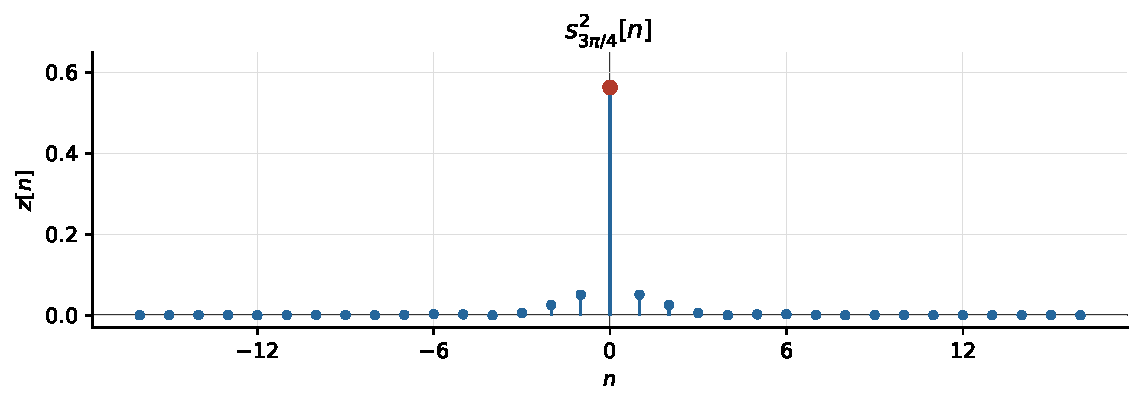
\includegraphics[width=0.82\textwidth]{07-dtft/examples/square-wide-given.pdf}
    \caption{例题 \ref{ex:dtft-sinc-square-wide} 的宽 sinc 平方，$z[0]=9/16$。}
    \label{fig:ex-dtft-square-wide-given}
  \end{figure}
\end{workedexample}

\begin{solution}
  \textbf{方法一：普通卷积后周期叠加。}
  两个半宽 $3\pi/4$ 的单位矩形做普通卷积得到
  \[
    C_0(\omega)=(3\pi/2-|\omega|)_+.
  \]
  三角形的端点为 $\pm3\pi/2$，超过主周期边界。对 $|\omega|\le\pi/2$，相邻副本不进入，只有 $C_0(\omega)$。对 $\pi/2\le\omega\le\pi$，右侧副本的贡献为
  \[
    C_0(\omega-2\pi)=3\pi/2-(2\pi-\omega)=\omega-\pi/2.
  \]
  它与中央的 $3\pi/2-\omega$ 相加恰为 $\pi$。负频率区由偶对称得到相同结果。乘 $1/(2\pi)$，
  \[
    \boxed{Z(\e^{\iu\omega})=
      \begin{cases}
        \displaystyle\frac34-\frac{|\omega|}{2\pi},
            &|\omega|\le\pi/2,\\
        \displaystyle\frac12,&\pi/2<|\omega|\le\pi.
      \end{cases}}
  \]
  外侧平台来自重叠，不能画成零。\cref{fig:ex-dtft-square-wide-folding} 显示三份普通三角形及其相加结果。
  \begin{figure}[H]
    \centering
    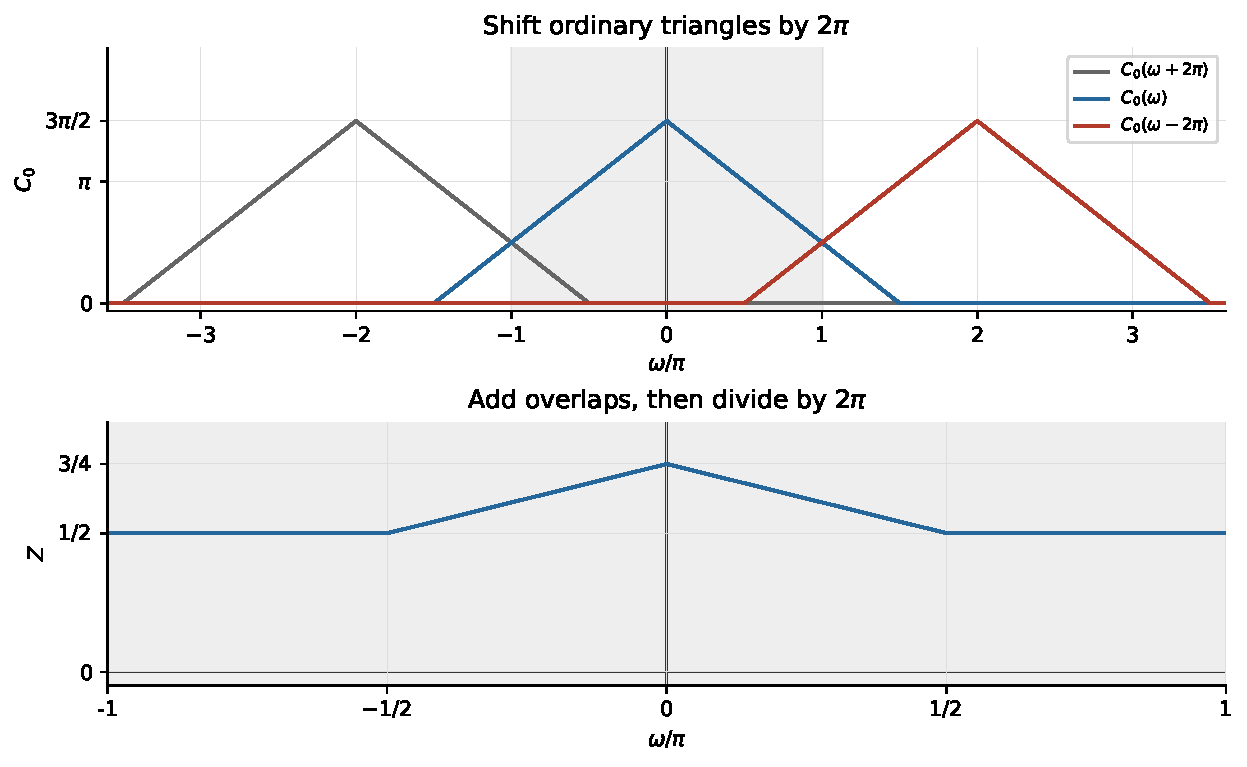
\includegraphics[width=0.92\textwidth]{07-dtft/examples/square-wide-folding.pdf}
    \caption{例题 \ref{ex:dtft-sinc-square-wide} 的周期叠加。相邻副本在主周期两侧补入，使两侧的和为常数 $\pi$；归一化后平台为 $1/2$。}
    \label{fig:ex-dtft-square-wide-folding}
  \end{figure}

  \textbf{方法二：非零样值化简后补零点。}
  对非零整数 $n$，
  \[
    \sin(3\pi n/4)=\sin(\pi n-\pi n/4)
       =(-1)^{n+1}\sin(\pi n/4).
  \]
  平方后符号消失，两个序列在 $n\ne0$ 处相同；零点差为 $9/16-1/16=1/2$，所以
  \[
    s_{3\pi/4}^2[n]=s_{\pi/4}^2[n]+\frac12\impulse[n].
  \]
  频谱即窄三角形加常数 $1/2$，与方法一一致，见\cref{fig:ex-dtft-square-wide-answer}。面积为
  $\pi+\pi/8=9\pi/8$，除以 $2\pi$ 得 $9/16$；零频值为 $3/4$，也符合 $\sum_n s_{3\pi/4}^2[n]=3/4$。
  \begin{figure}[H]
    \centering
    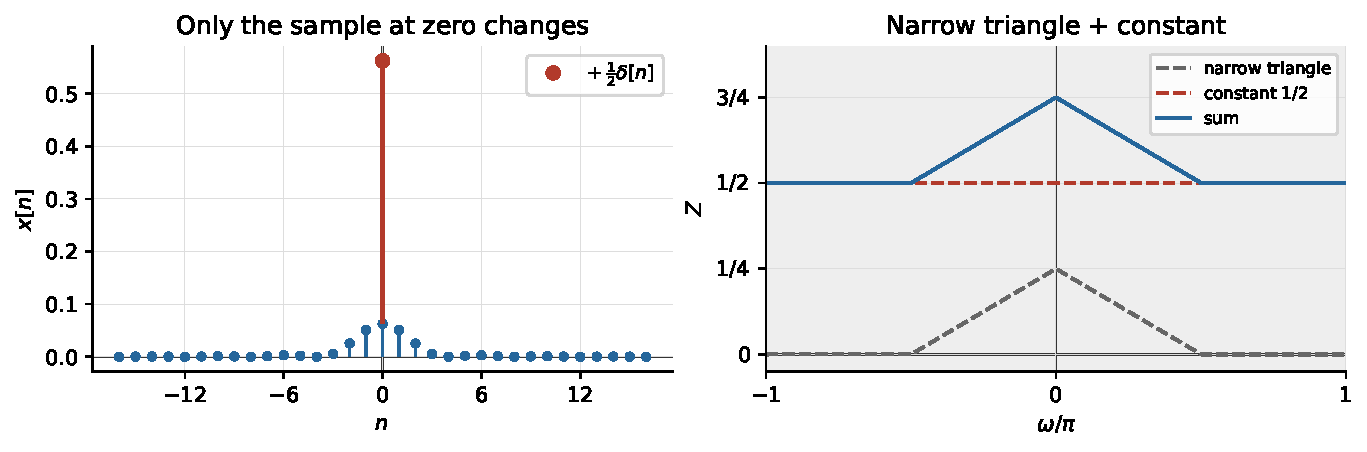
\includegraphics[width=0.90\textwidth]{07-dtft/examples/square-wide-answer.pdf}
    \caption{例题 \ref{ex:dtft-sinc-square-wide} 的另一种表示：窄三角频谱加常数 $1/2$，等价于时域只增加零点样值。}
    \label{fig:ex-dtft-square-wide-answer}
  \end{figure}
\end{solution}

\begin{technique}
  周期卷积先画普通卷积，再按 $2\pi$ 平移，逐段确定进入主周期的副本。若能化简整数位置上的正弦，也要在化简后检查零点；非零位置相同的两序列，仍可能相差一个单位冲激。
\end{technique}

\begin{workedexample}[由频谱虚部、单侧条件与能量恢复序列]
  \label{ex:dtft-imaginary-energy-recovery}
  已知 $x[n]$ 是实序列，满足 $x[n]=0$（$n>0$）、$x[0]>0$，且
  \[
    \Im X(\e^{\iu\omega})=\sin\omega-\sin2\omega,\qquad
    \int_{-\pi}^{\pi}|X(\e^{\iu\omega})|^2\dd\omega=6\pi.
  \]
  求 $x[n]$。已知虚部见\cref{fig:ex-dtft-recovery-given}。
  \begin{figure}[H]
    \centering
    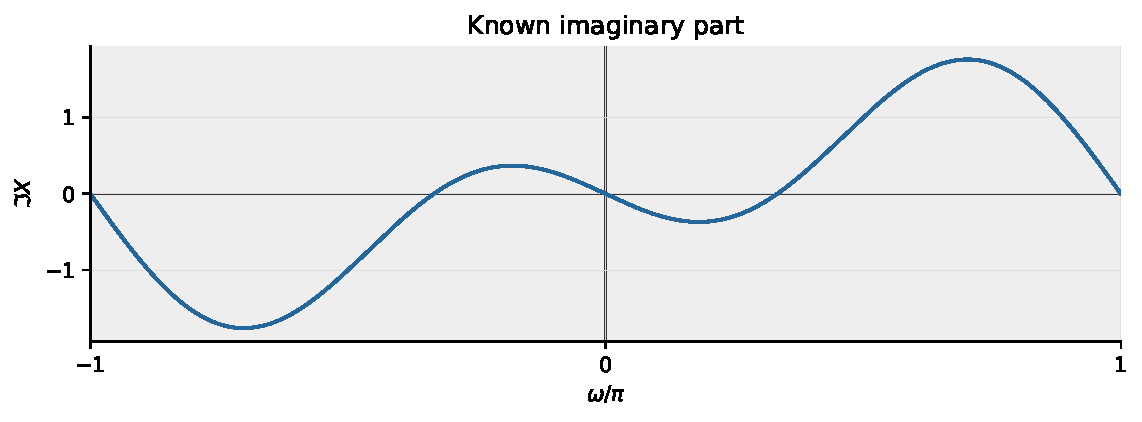
\includegraphics[width=0.82\textwidth]{07-dtft/examples/recovery-given.pdf}
    \caption{例题 \ref{ex:dtft-imaginary-energy-recovery} 的频谱虚部。它为奇函数，与实序列的共轭对称条件一致。}
    \label{fig:ex-dtft-recovery-given}
  \end{figure}
\end{workedexample}

\begin{solution}
  先由虚部求奇分量。按照\cref{eq:dtft-even-odd-spectrum}，
  \begin{align*}
    x_{\mathrm o}[n]&\fourierpair
       \iu(\sin\omega-\sin2\omega)\\
      &=\frac12\e^{\iu\omega}-\frac12\e^{-\iu\omega}
        -\frac12\e^{2\iu\omega}+\frac12\e^{-2\iu\omega}.
  \end{align*}
  用时移冲激 $\impulse[n-n_0]\fourierpair\e^{-\iu\omega n_0}$ 逐项反演，
  \[
    x_{\mathrm o}[n]
      =\frac12\impulse[n+1]-\frac12\impulse[n-1]
        -\frac12\impulse[n+2]+\frac12\impulse[n-2].
  \]
  先画出正负下标各点，再用单侧条件恢复，见\cref{fig:ex-dtft-recovery-alignment}。对 $n<0$，$x[-n]=0$，故 $x[n]=2x_{\mathrm o}[n]$；于是
  \[
    x[-2]=-1,\qquad x[-1]=1,\qquad x[n]=0\quad(n\le-3).
  \]
  奇分量在 $n=0$ 恒为零，尚不能确定 $x[0]$。记 $A=x[0]>0$，则
  \[
    x[n]=-\impulse[n+2]+\impulse[n+1]+A\impulse[n].
  \]
  \begin{figure}[H]
    \centering
    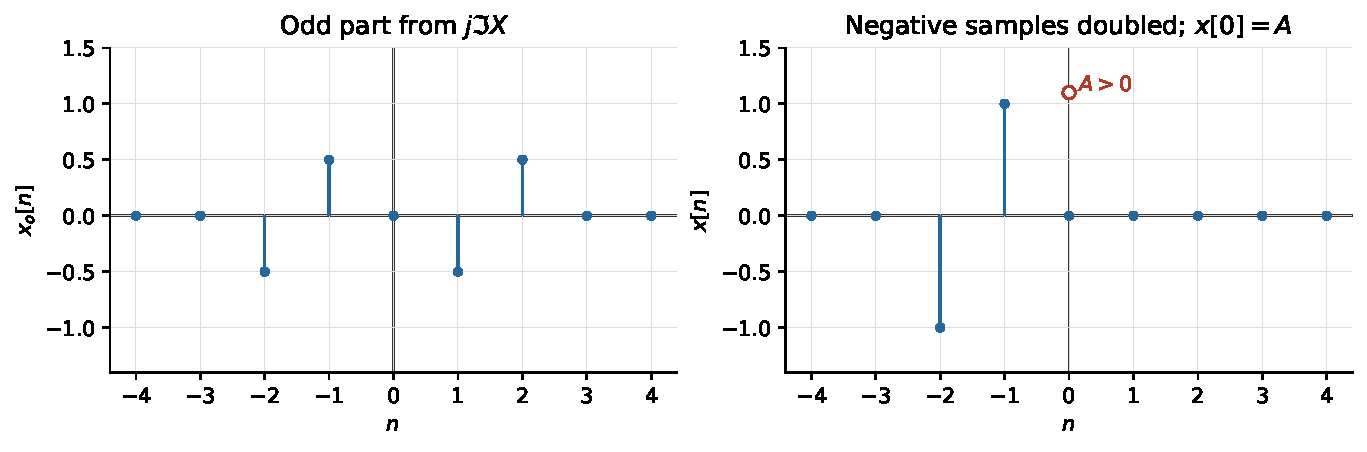
\includegraphics[width=0.90\textwidth]{07-dtft/examples/recovery-alignment.pdf}
    \caption{例题 \ref{ex:dtft-imaginary-energy-recovery}：先反演奇分量，再把负下标样值加倍；零点样值另由能量确定。}
    \label{fig:ex-dtft-recovery-alignment}
  \end{figure}

  帕塞瓦尔定理给出 $E=6\pi/(2\pi)=3$，所以
  \[
    (-1)^2+1^2+A^2=3,\qquad A>0
    \quad\Longrightarrow\quad A=1.
  \]
  最终
  \[
    \boxed{x[n]=\impulse[n]+\impulse[n+1]-\impulse[n+2]}.
  \]
  正变换核对：
  \[
    X(\e^{\iu\omega})=1+\e^{\iu\omega}-\e^{2\iu\omega},
    \quad \Re X=1+\cos\omega-\cos2\omega,\quad
    \Im X=\sin\omega-\sin2\omega.
  \]
  三个非零样值的能量为 $3$，共轭对称与给定虚部均成立；答案见\cref{fig:ex-dtft-recovery-answer}。
  \begin{figure}[H]
    \centering
    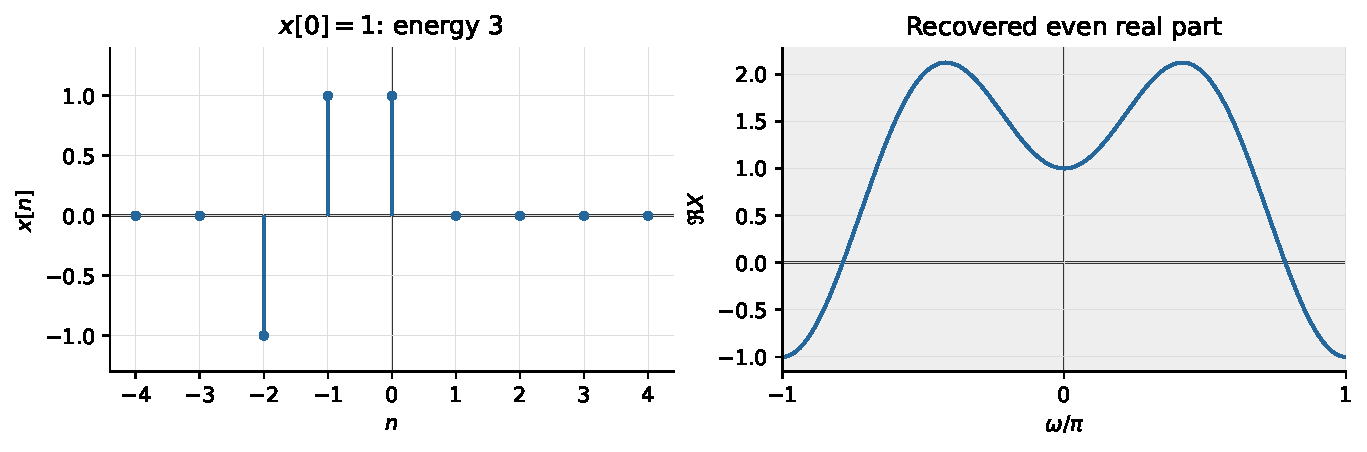
\includegraphics[width=0.90\textwidth]{07-dtft/examples/recovery-answer.pdf}
    \caption{例题 \ref{ex:dtft-imaginary-energy-recovery} 的恢复序列与频谱实部。实部补齐了虚部无法确定的偶分量。}
    \label{fig:ex-dtft-recovery-answer}
  \end{figure}
\end{solution}

\begin{technique}
  先确认实序列条件，再将 $\iu\Im X$ 拆成复指数以反演奇分量。单侧条件决定一侧样值与奇分量之间的倍数，零点由能量补足；若没有 $x[0]>0$，本题只能确定 $x[0]=\pm1$。
\end{technique}
\endgroup
